\section{SM and Higgs results}
\label{section_sm_higgs}

The Standard Model have been proven extremely successful in describing what it is proposed to do. The discovery of the two highest invariant mass particles of the SM, the top quark~\cite{top_discovery_cdf,top_discovery_d0}, by the CDF and 0 collaboration, at FERMILAB, and the Higgs Boson~\cite{higgs_discovery_cms,higgs_discovery_atlas}, by CMS and ATLAS, at CERN, fill the two missing pieces of the SM puzzle, presented at Figure~\ref{sm_summary}. In general, SM measurements presents very good agreement between theory and experiment, even when the Higgs boson is taken into account, once it mass has been established, the subsequent results tend to be found restricted within the expectations and constrained by the statistics and experimental sensitivity.  

In this section, we shall briefly review some of the most relevant SM results from LHC, with special focus to $Z$ and Higgs boson, subjects of the study. 


\begin{sidewaysfigure}[htbp]
  \centering
  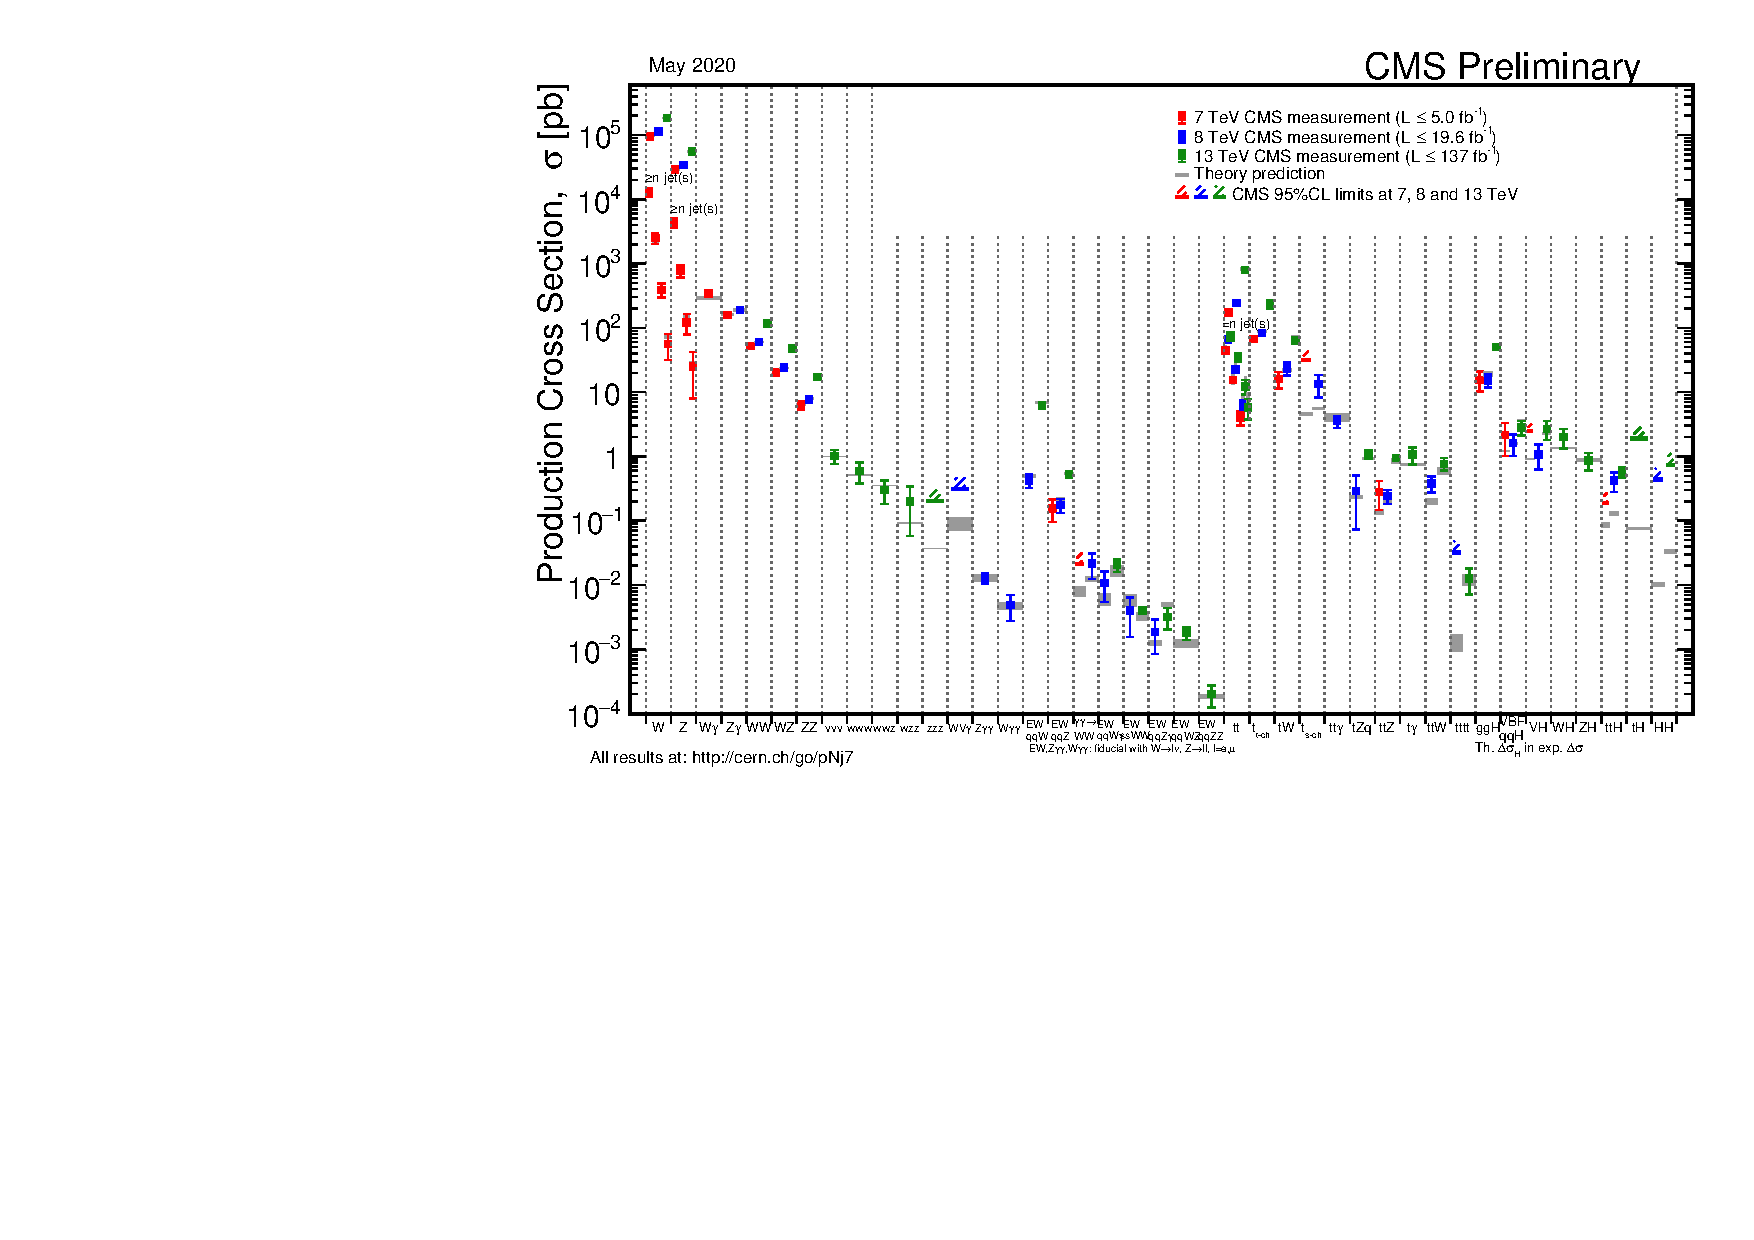
\includegraphics[width=\textwidth]{figures_and_tables/theory/cms_sm_xsec.pdf}
  \caption{\todo{SM x-sec!!!!!} Summary of the cross section measurements of Standard Model processes at CMS. Source:~\cite{cms_sm_xsec_summary}.}
  \label{cms_sm_xsec}
\end{sidewaysfigure}

\begin{figure}[htbp]
  \centering
  \begin{subfigure}[htbp]{0.48\textwidth}
    \centering
    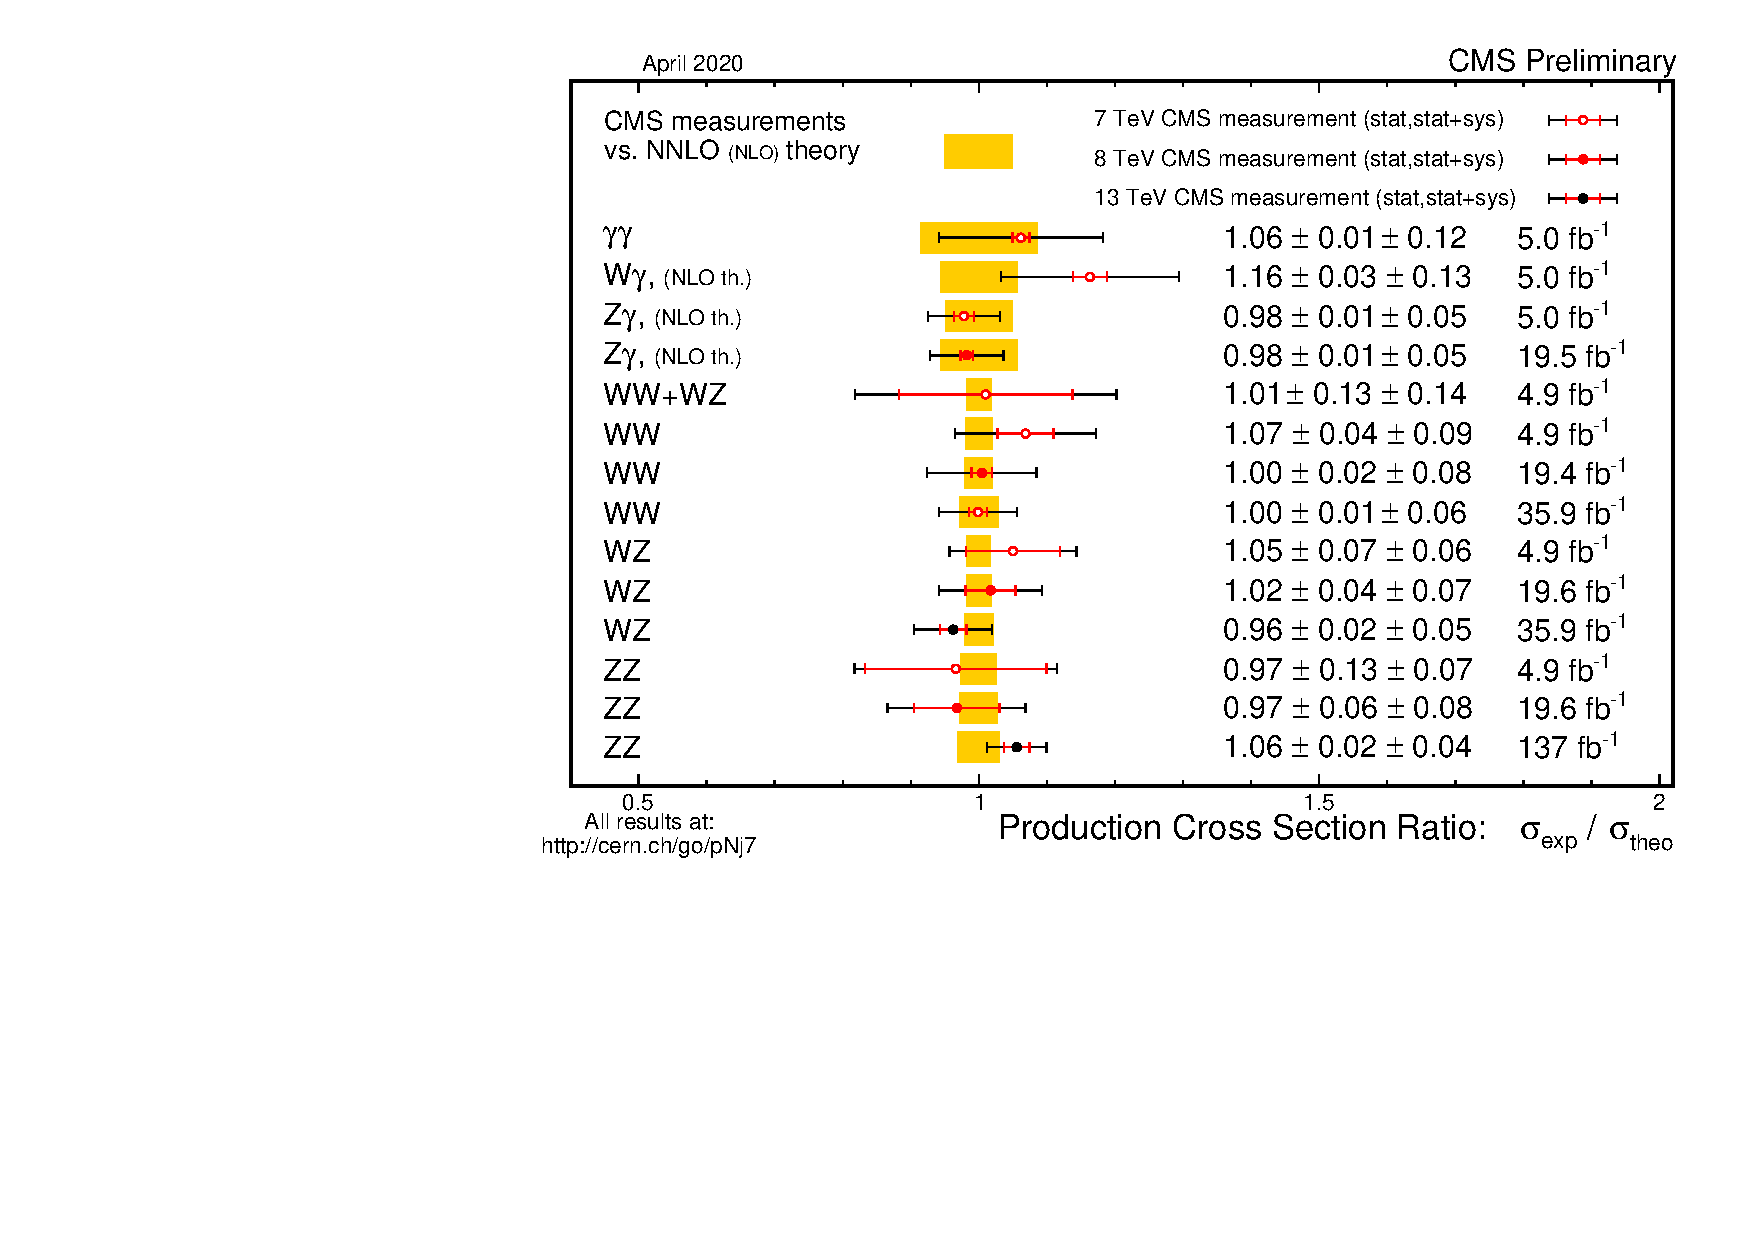
\includegraphics[width=\textwidth]{figures_and_tables/theory/sm_vbf_results.pdf}
    \caption{\todo{Expanadir!} Di-boson cross section ratio comparison to theory: Theory predictions updated to latest NNLO calculations where available compared to predictions in the CMS papers and preliminary physics analysis summaries. Source:~\cite{cms_sm_xsec_summary}.}
  \label{sm_vbf_results}
  \end{subfigure}
  \hfill
  \begin{subfigure}[htbp]{0.48\textwidth}
    \centering
    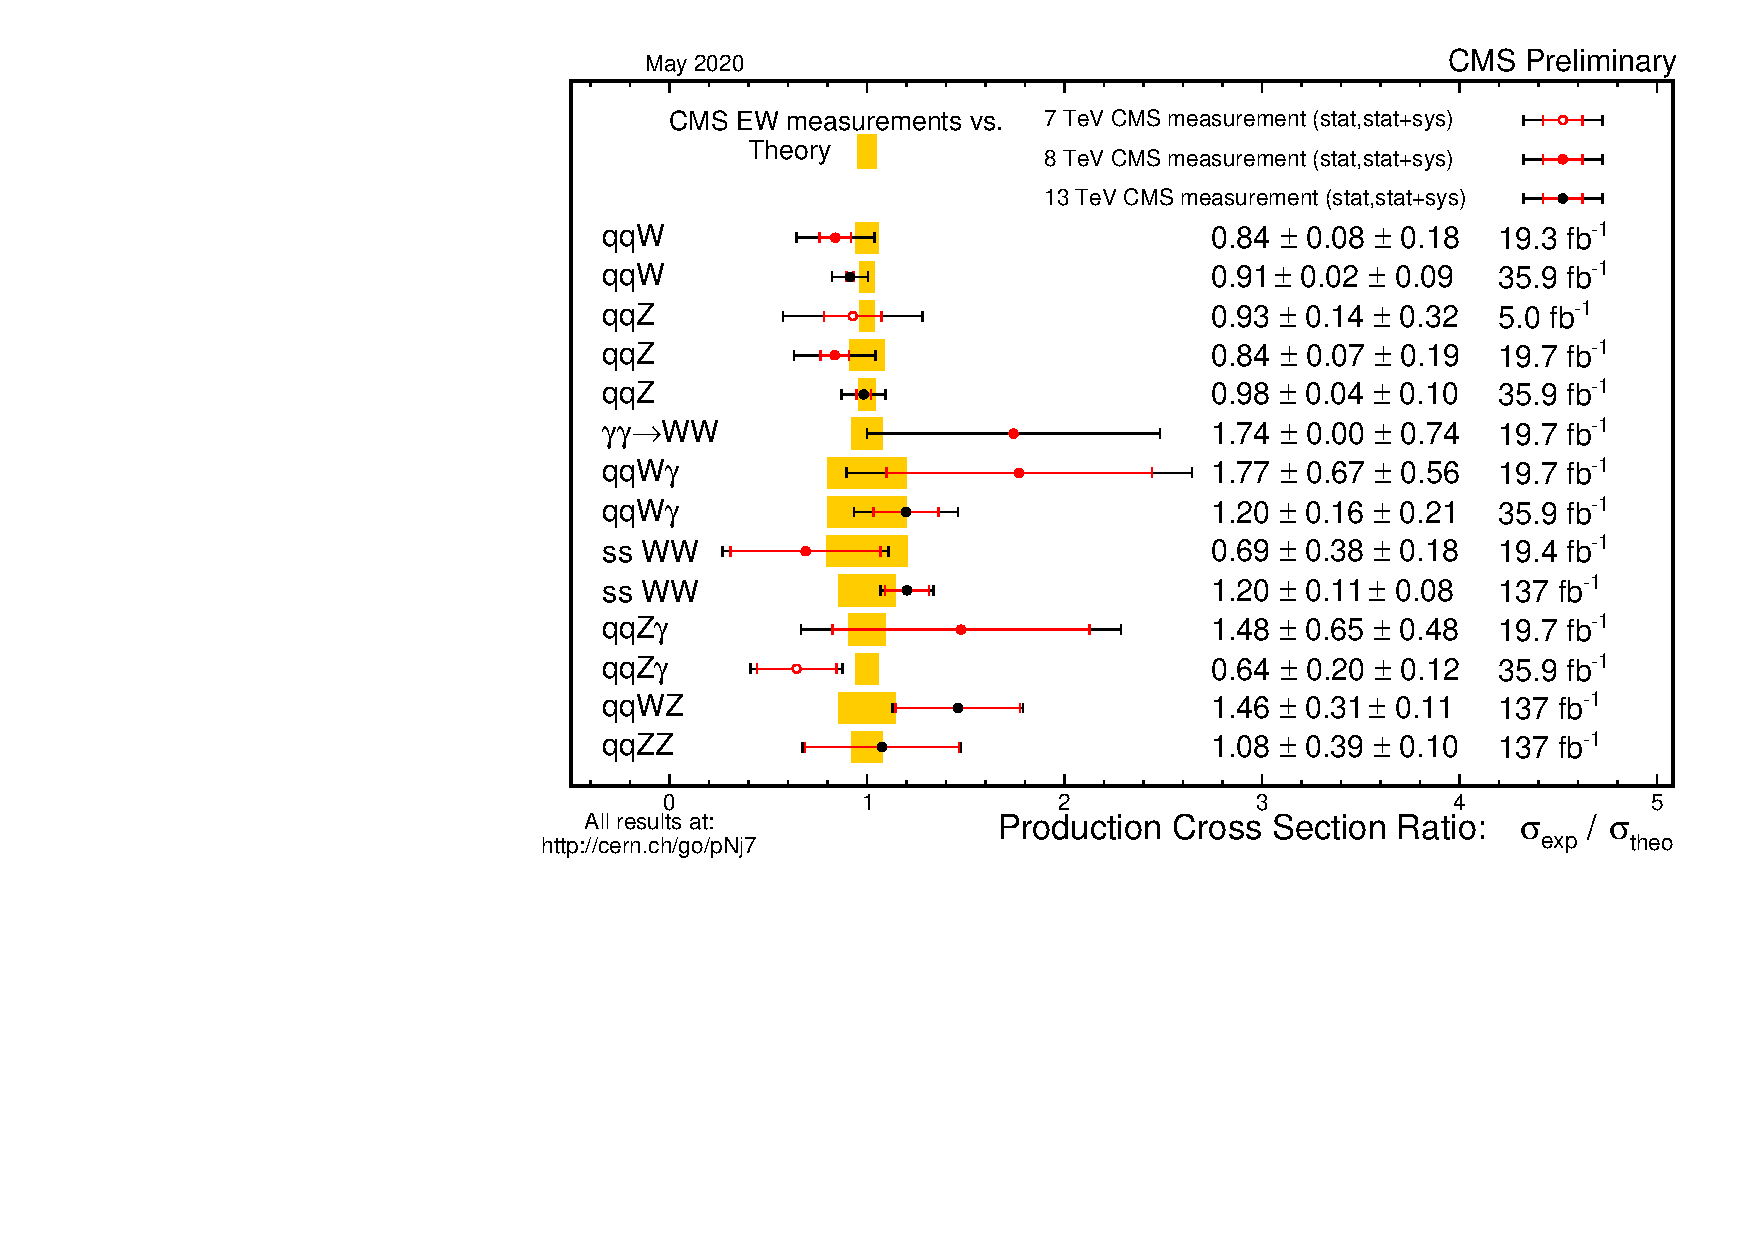
\includegraphics[width=\textwidth]{figures_and_tables/theory/sm_ewk_results.pdf}
    \caption{\todo{Expanadir!} Summary of the cross sections of pure Electroweak (EWK) interactions among the gauge bosons presented as a ratio compared to theory. Source:~\cite{cms_sm_xsec_summary}.}
    \label{sm_ewk_results}
  \end{subfigure}
\end{figure}

\todo{Higgs}

\todo{discovery}
\todo{Production modes}
\todo{Decay modes}

\begin{figure}[htbp]
  \centering
  \begin{subfigure}[htbp]{0.48\textwidth}
    \centering
    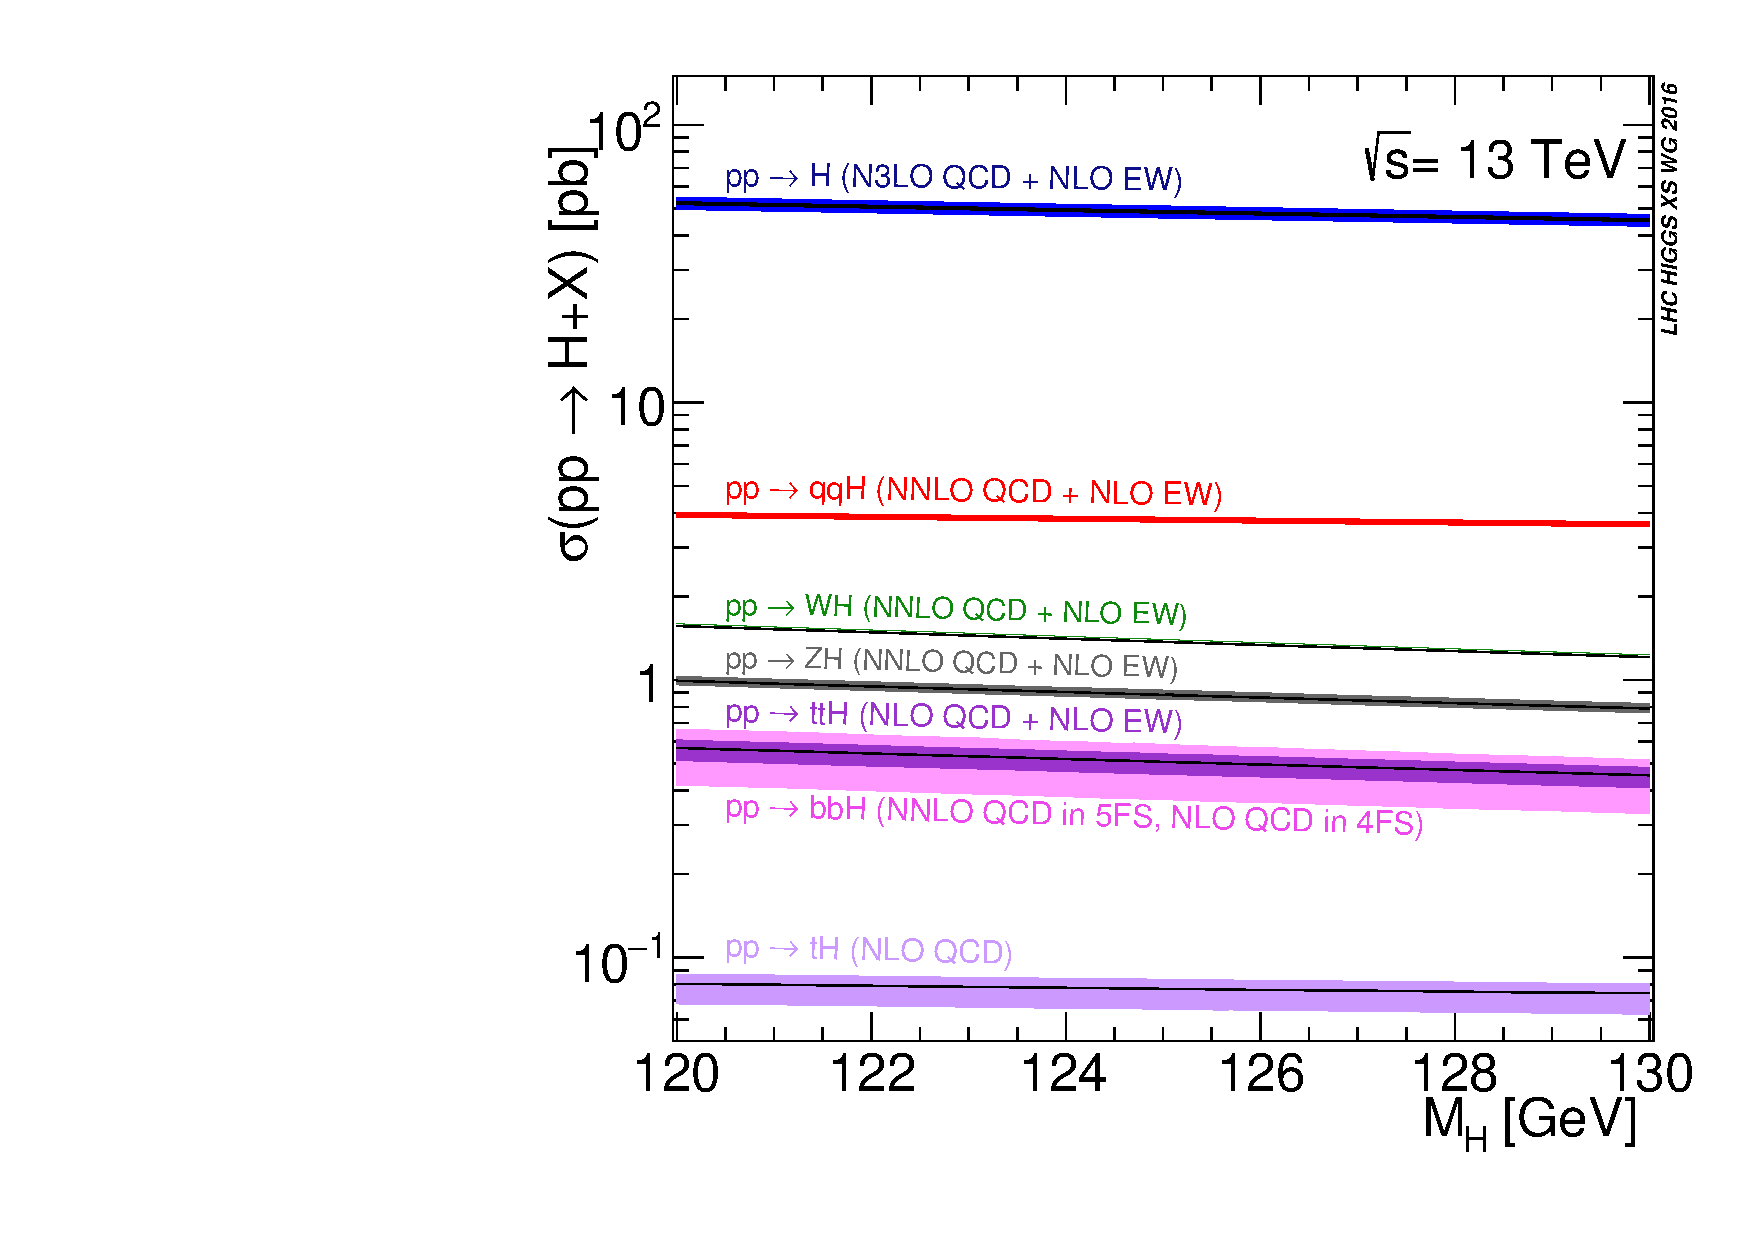
\includegraphics[width=\textwidth]{figures_and_tables/theory/higgs_prod_modes.pdf}
    \caption{\todo{Exapandir!}  Standard Model Higgs boson production cross sections at $\sqrt{s}=13$ TeV as a function of Higgs boson mass. The tH production cross section accounts for $t$-channel and $s$-channel only (no $tWH$ production). Source:~\cite{deFlorian:2016spz}.}
  \label{higgs_prod_modes}
  \end{subfigure}
  \hfill
  \begin{subfigure}[htbp]{0.48\textwidth}
    \centering
    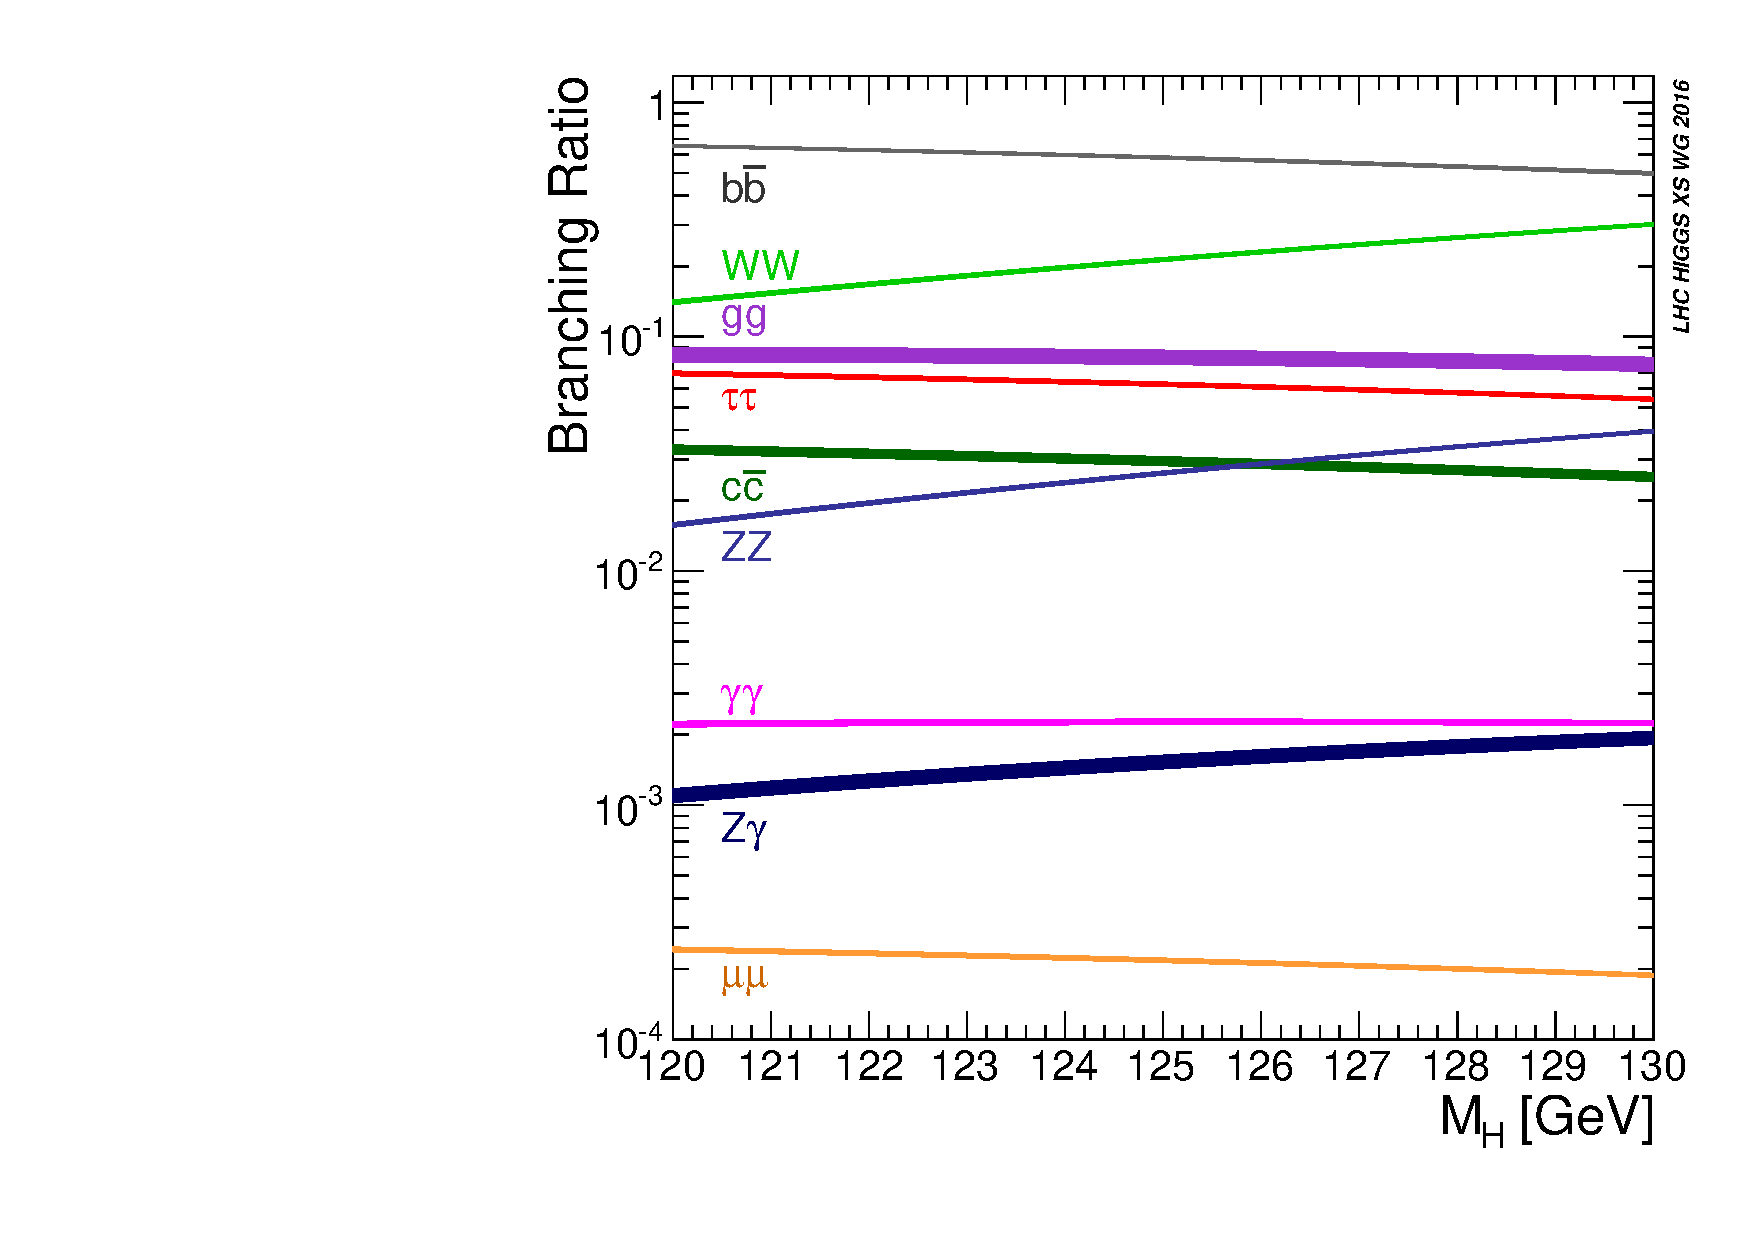
\includegraphics[width=\textwidth]{figures_and_tables/theory/higgs_decays.pdf}
    \caption{\todo{Exapandir!} Standard Model Higgs boson decay branching ratios for each decays channel. Source:~\cite{deFlorian:2016spz}.}
    \label{higgs_decays}
  \end{subfigure}
\end{figure}

\todo{Yukawa coupling}

\todo{Higgs results at CMS}

% Higgs discovery
\begin{figure}[htbp]
  \centering
  \begin{subfigure}[htbp]{0.48\textwidth}
    \centering
    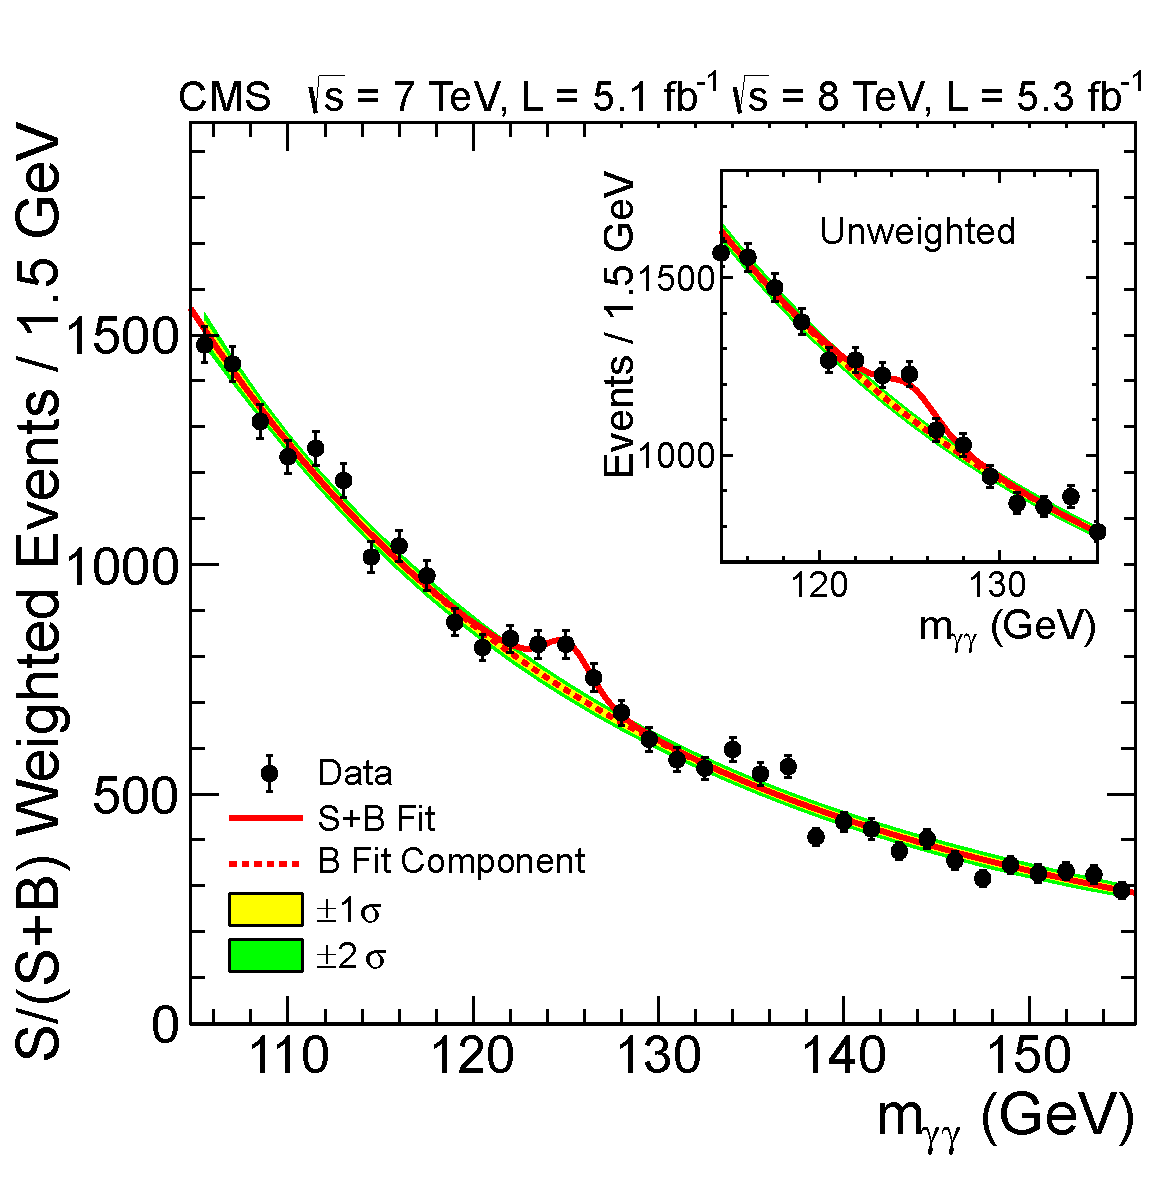
\includegraphics[width=\textwidth]{figures_and_tables/theory/higgs_discovery_hgg.pdf}
    \caption{\todo{Exapandir!} The diphoton invariant-mass distribution for the 7 and 8 \TeV datasets (points), with each event weighted by the predicted $S/(S+B)$ ratio of its event class. The solid and dotted lines give the results of the signal-plus-background and background-only fit, respectively. The light and dark bands represent the $\pm$1 and $\pm$2 standard deviation uncertainties respectively on the background estimate. The inset shows the corresponding unweighted invariant-mass distribution around \mbox{$m_{\gamma\gamma}$ = 125 \GeV}. Source:~\cite{higgs_discovery_cms}.}
  \label{higgs_discovery_hgg}
  \end{subfigure}
  \hfill
  \begin{subfigure}[htbp]{0.48\textwidth}
    \centering
    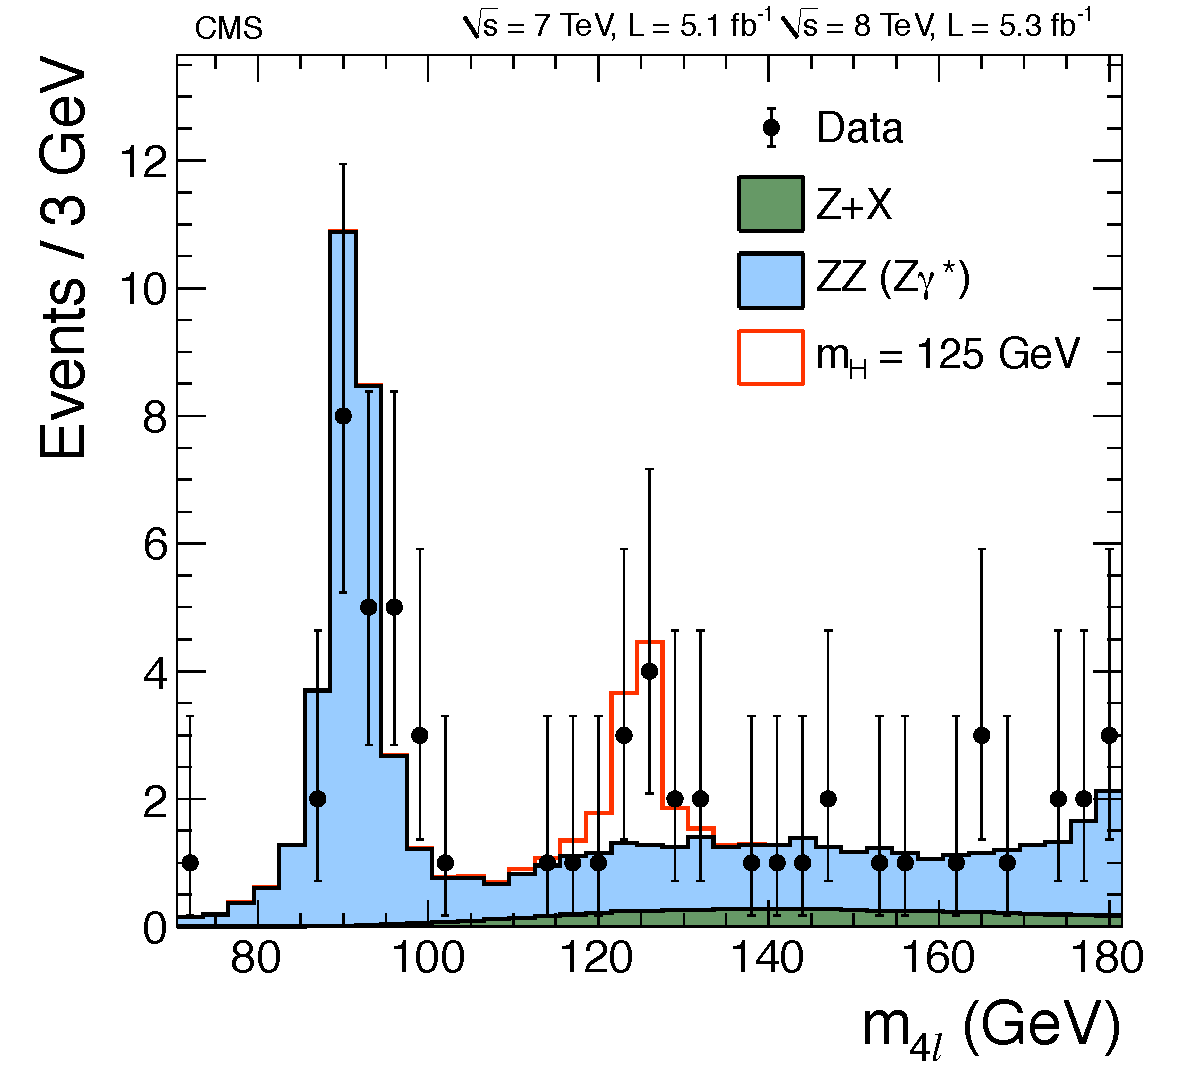
\includegraphics[width=\textwidth]{figures_and_tables/theory/higgs_discovery_hzz4l.pdf}
    \caption{\todo{Exapandir!} Distribution of the observed four-lepton invariant mass from the combined 7 and 8 \TeV data 
    for the $\PH \to \cPZ\cPZ\to 4\ell$ analysis (points).
    The prediction for the expected $\cPZ$+X and $\cPZ\cPZ(\cPZ\gamma^*)$ background are shown by the dark and light histogram, respectively. The open histogram gives the expected distribution for a Higgs boson of mass 125 \GeV. Source:~\cite{higgs_discovery_cms}.}
    \label{higgs_discovery_hzz4l}
  \end{subfigure}
\end{figure}




% signal strength modifier - COMB RUn2
\begin{figure}[htbp]
  \centering
  \begin{subfigure}[htbp]{0.48\textwidth}
    \centering
    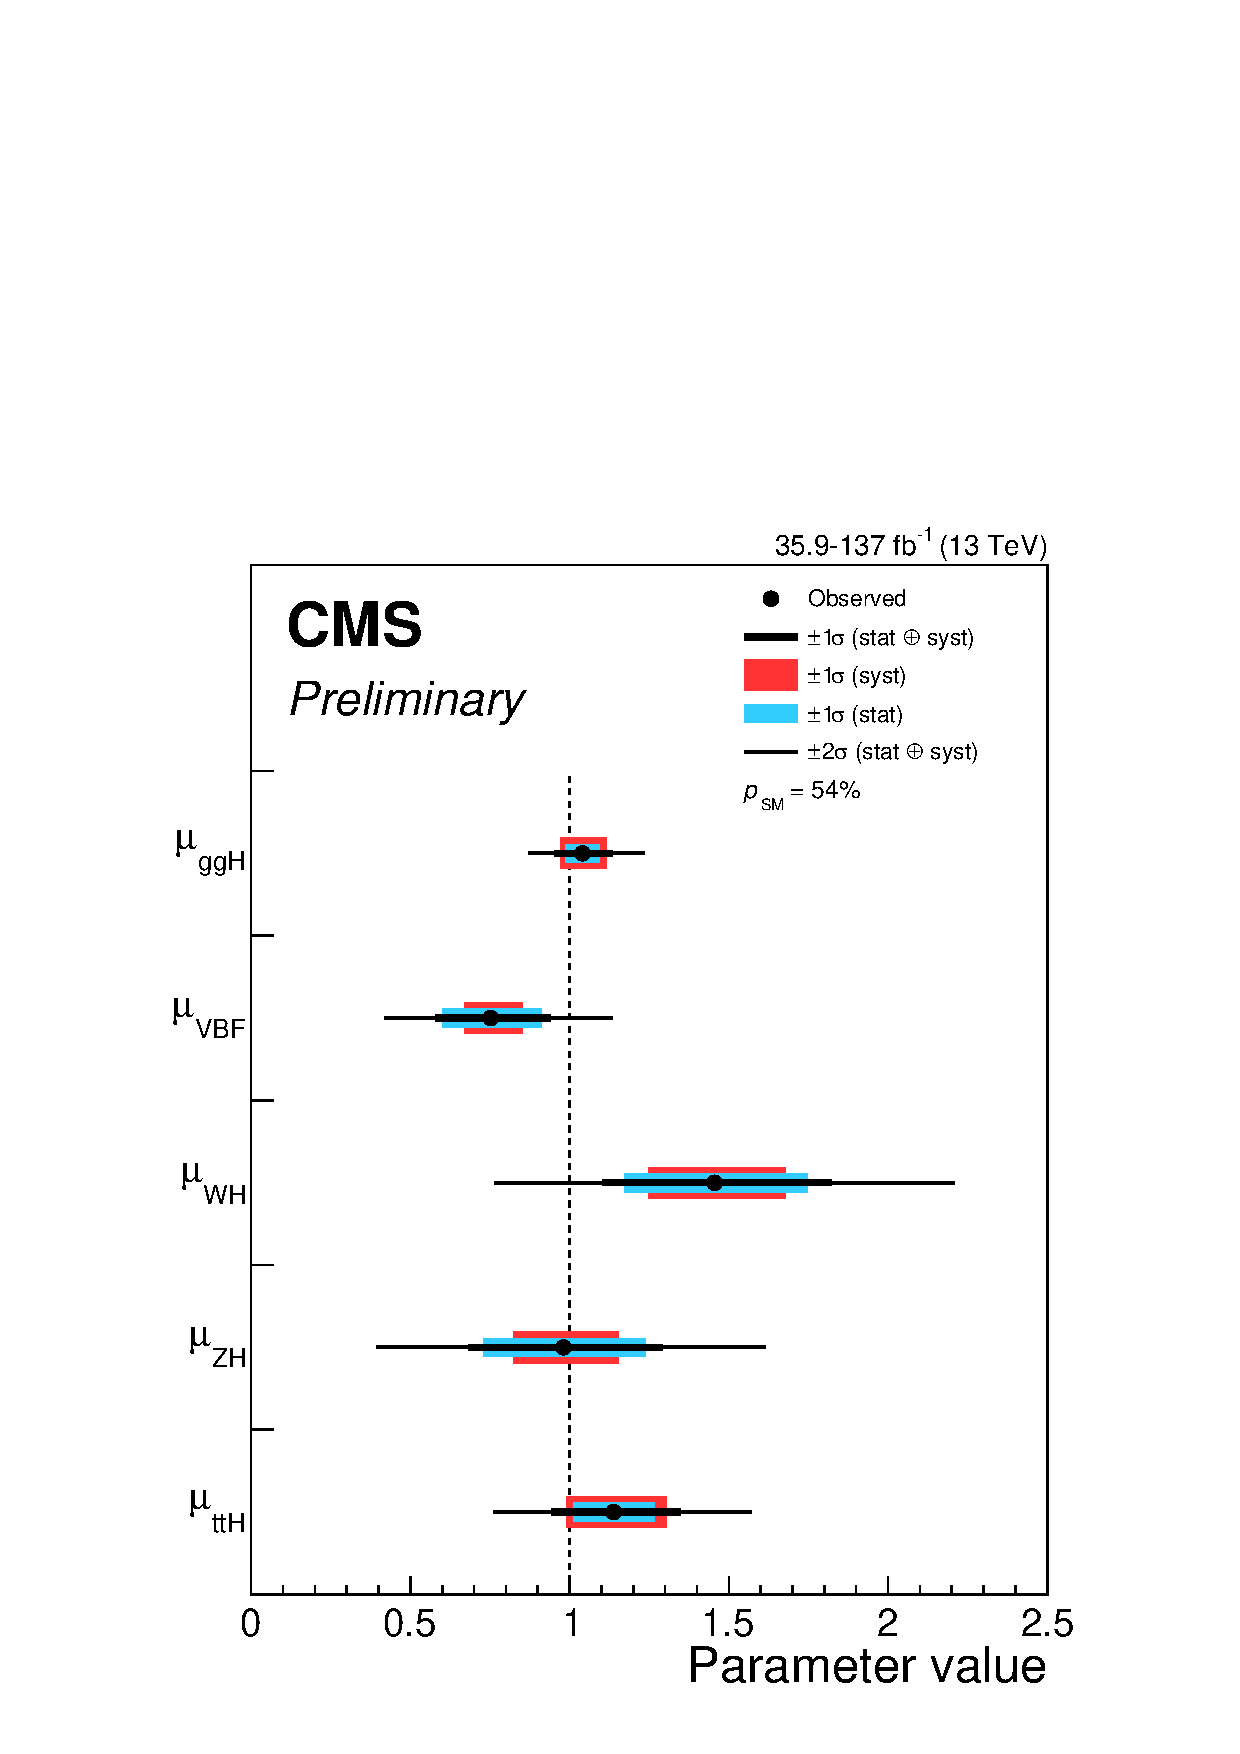
\includegraphics[width=\textwidth]{figures_and_tables/theory/signal_strength_modifier_prod.pdf}
    \caption{ }
  \label{signal_strength_modifier_prod}
  \end{subfigure}
  \hfill
  \begin{subfigure}[htbp]{0.48\textwidth}
    \centering
    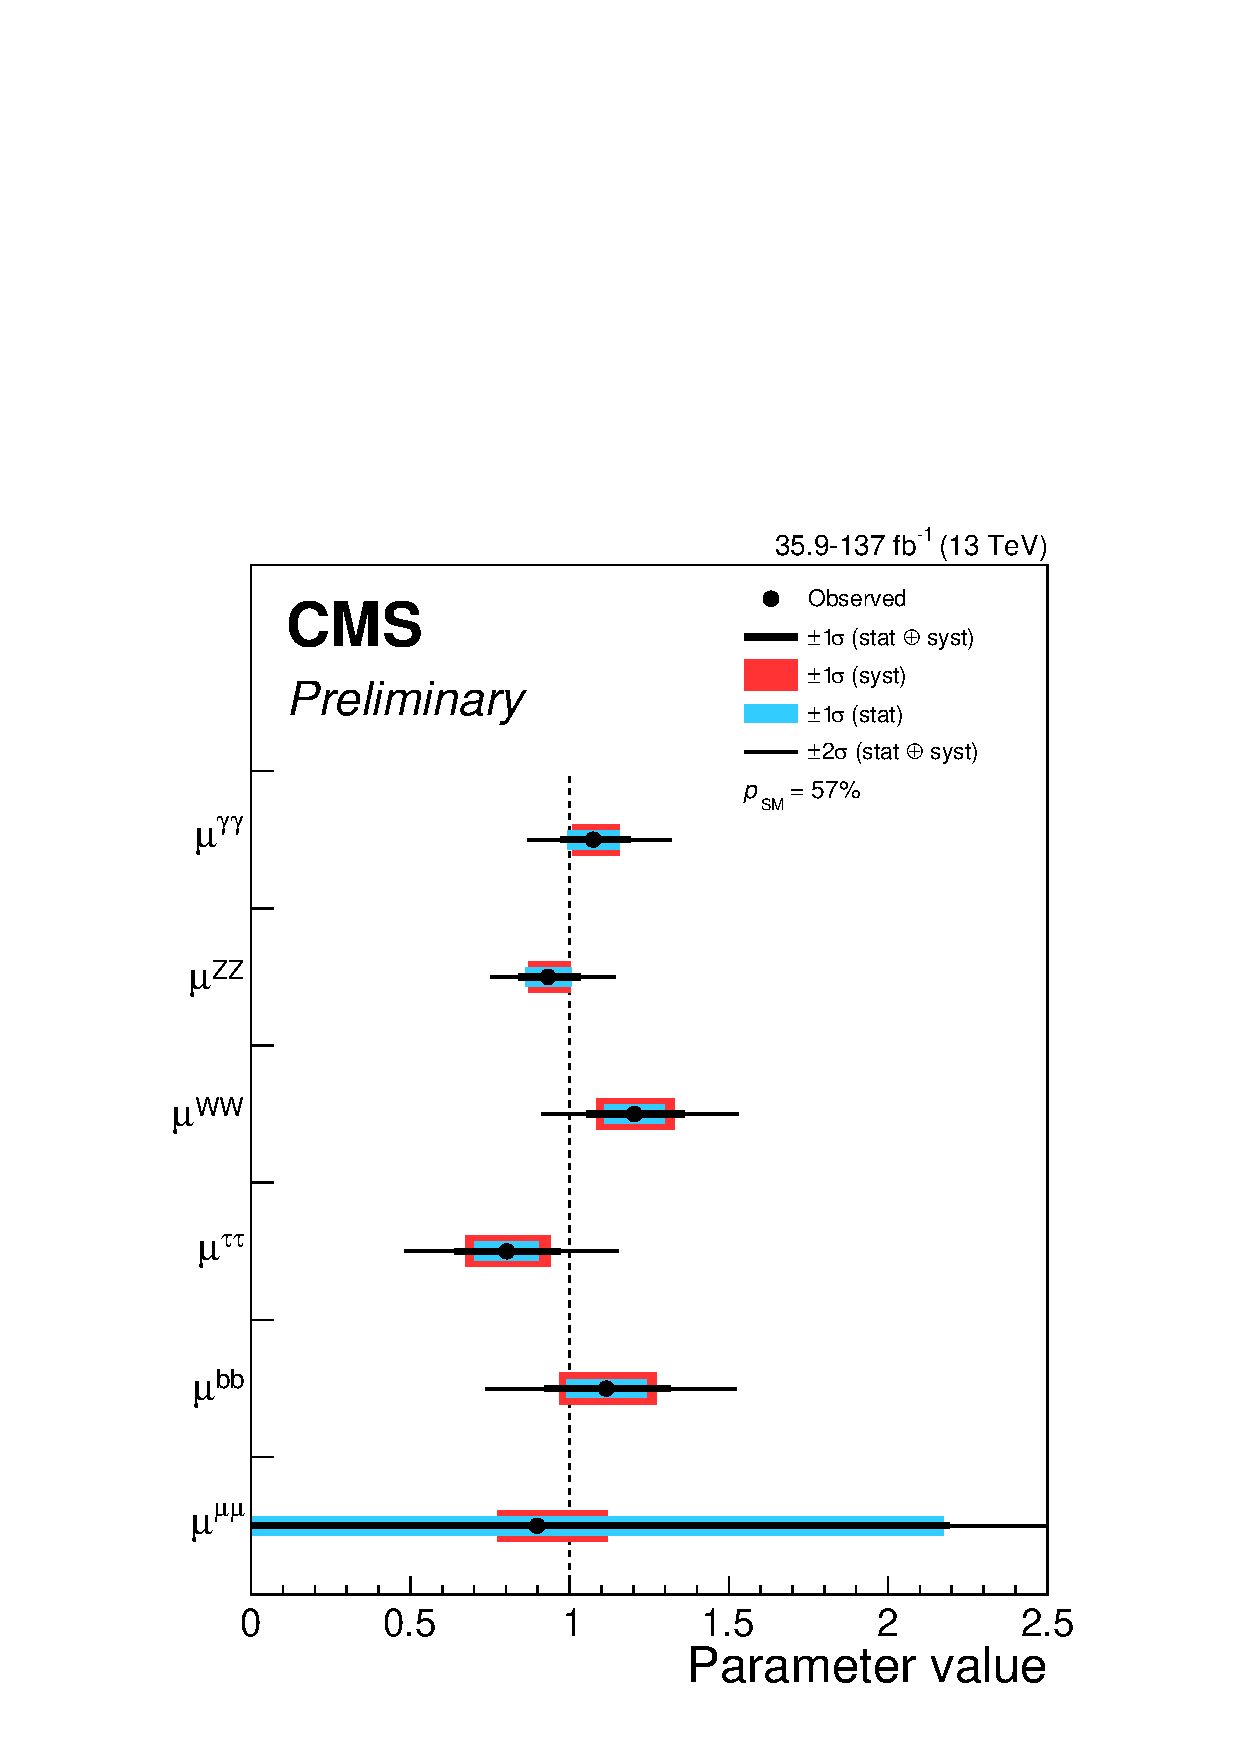
\includegraphics[width=\textwidth]{figures_and_tables/theory/signal_strength_modifier_decay.pdf}
    \caption{ }
    \label{signal_strength_modifier_decay}
  \end{subfigure}
  \caption{\todo{Expandir!} Signal strength modifiers for the production, $\mu^{i}$, and for the decay, $\mu^{f}$, modes on the left and the right panel, respectively. The thick (thin) black lines report the $1\sigma$ ($2\sigma$) confidence intervals. The thick blue and red lines report the statistical and systematic components of the $1\sigma$ confidence intervals. The assumptions used in this fit are described in the text. Source:~\cite{cms_higgs_comb_run2}.}
\end{figure}





% H to mumu
\begin{figure}[htbp]
  \centering
  \begin{subfigure}[htbp]{0.48\textwidth}
    \centering
    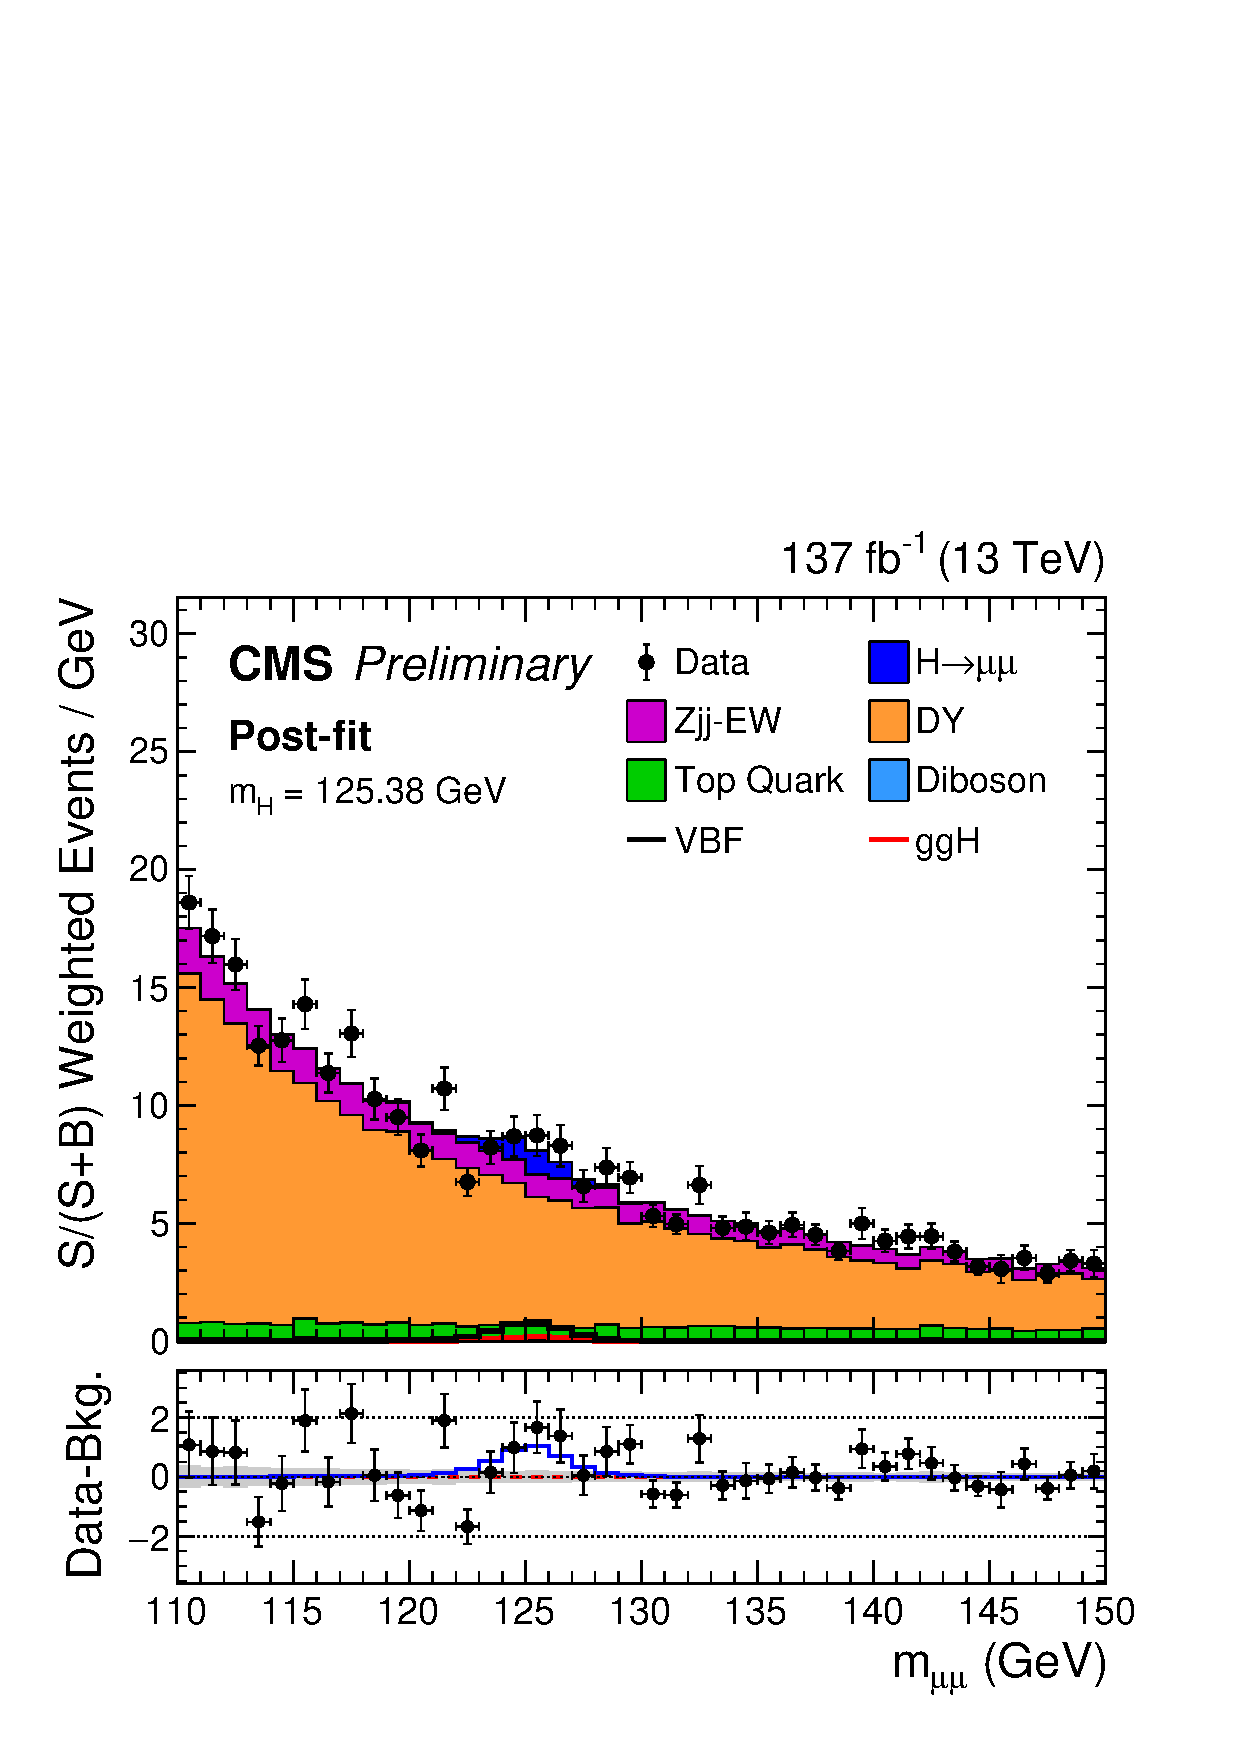
\includegraphics[width=\textwidth]{figures_and_tables/theory/h_to_mumu_result.pdf}
    \caption{\todo{Higgs to MuMu. É apenas um evidência!} The $m_{\mu\mu}$ distribution for the weighted combination of VBF events. Each event is weighted proportionally to the $S/(S + B)$ ratio. The lower panel shows the residuals after subtracting the background prediction from the signal-plus-background fit. The best-fit $H \rightarrow \mu\mu$ signal contribution is indicated by the blue line, and the grey band indicates the total background uncertainty from the background-only fit. The measured signal strength is ${1.19^{+0.41}_{-0.39}(\mathrm{stat})^{+0.17}_{-0.16}(\mathrm{sys})}$. Source:~\cite{cms_higgs_mumu}.}
  \label{h_to_mumu_result}
  \end{subfigure}
  \hfill
  \begin{subfigure}[htbp]{0.48\textwidth}
    \centering
    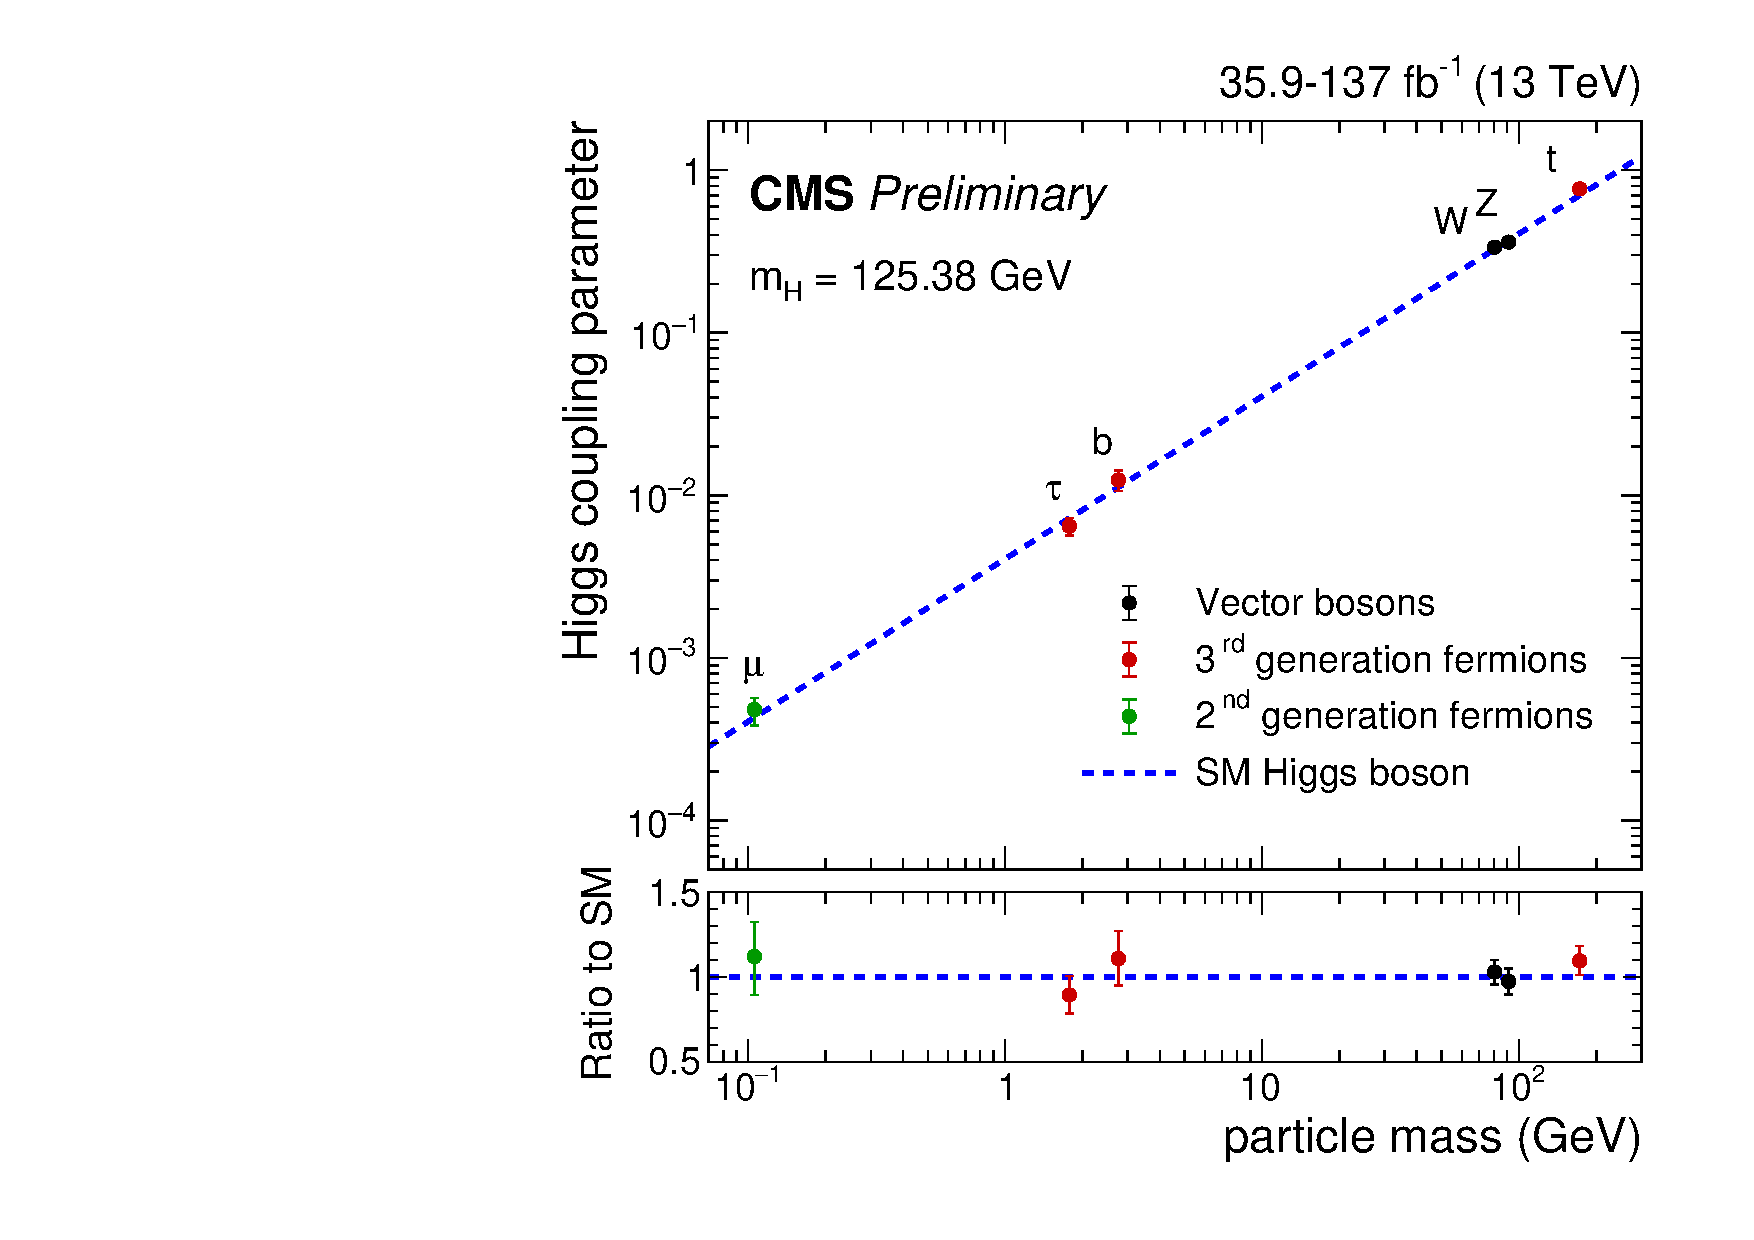
\includegraphics[width=\textwidth]{figures_and_tables/theory/higgs_coups.pdf}
    \caption{\todo{Higgs to MuMu. É apenas um evidência!} The best-fit estimates for the reduced coupling modifiers extracted for fermions and weak bosons from the resolved $\kappa$-framework model compared to their corresponding prediction from the SM. The error bars represent 68\% CL intervals for the measured parameters. The lower panel shows the ratios of the measured coupling modifiers values to their SM predictions. Source:~\cite{cms_higgs_mumu}.}
    \label{higgs_coups}
  \end{subfigure}
\end{figure}

